\titleformat{\chapter}[hang]{\Huge\bfseries}{\selectfont \thechapter\hsp\textcolor{red}{\emoji{open-book}}\hsp}{0pt}{\Huge\bfseries}

\chapter{Data Understanding}

This chapter covers the data understanding phase of the CRISP-DM methodology.

\section{Collect Initial Data}

The available data are being collected from the social network platform Gab\footnote{\url{https://gab.com/}}. The dataset includes several snapshots, in particular, \texttt{2016-2021}, \texttt{2022}, \texttt{2023}, \texttt{2024}, \texttt{January-July 2025} and \texttt{July 2025}. For every snapshot, there three files:

\begin{itemize}
	\item \texttt{posts\_current\_snapshot.csv}: contains all the posts made by users in the platform for that snapshot;
	\item \texttt{posts\_incremental.csv}: contains all the posts made by users in the platform since the previous snapshots up to the current one;
	\item \texttt{social\_network.edg}: contains the social network graph in edge list format, where every line represents a directed edge from a follower to a followee (X follows Y).
\end{itemize}

Along with them, there are also 3 synthetic batches for the subsequent task of using the trained model on the original data to generate links.

\section{Describe Data}

Raw data files are in CSV format, with the exception of the social network graph which is in edge list format. For each post, the following attributes are available:

\begin{itemize}
	% \item \texttt{unnamed\_0} (autoincrement): index of the post, autoincremented
	\item \texttt{id} (integer): unique identifier of the post
	\item \texttt{content} (string): text of the post
	\item \texttt{account\_id} (integer): unique identifier of the user who made the post
	\item \texttt{created\_at} (string): ISO 8601 timestamp of when the post was created
	\item \texttt{language} (string): language code of the post
	\item \texttt{replies\_count} (integer): number of replies to the post
	\item \texttt{reblogs\_count} (integer): number of reblogs of the post
	\item \texttt{reactions\_counts} (string): JSON dictionary of reactions to the post
	\item \texttt{quotes\_count} (integer): number of quotes of the post
	\item \texttt{timestamp} (string): ISO 8601 timestamp of the post (\texttt{created\_at} + timezone)
\end{itemize}


\section{Explore Data}

% The exploration of the dataset involves analyzing temporal patterns, content characteristics, user engagement, and activity distributions across all snapshots.

\sethlcolor{cyan!60}
The dataset had been preprocessed before: posts lacking textual content, posts containing images or videos, and posts written in languages other than English were removed. HTML tags were also stripped from the remaining content.


\subsection*{Temporal Distribution}

The dataset spans from August 22, 2016 to August 2, 2025, covering a period of approximately 9 years. Table~\ref{tab:temporaldistribution} summarizes the temporal distribution across all snapshots.

\begin{table}[H]
	\centering
	\caption{Temporal distribution of posts across snapshots}
	\label{tab:temporaldistribution}
	\begin{tabular}{lrrr}
		\toprule
		\textbf{Snapshot} & \textbf{Posts} & \textbf{Time Span (days)} & \textbf{Max Gap (days)} \\
		\midrule
		2016-2021         & 18,926         & 1,957                     & 49                      \\
		2022              & 13,108         & 364                       & $<$1                    \\
		2023              & 13,376         & 364                       & $<$1                    \\
		2024              & 13,400         & 365                       & $<$1                    \\
		Jan-Jul 25        & 44,878         & 180                       & $<$1                    \\
		Jul 25            & 78,857         & 32                        & $<$1                    \\
		\bottomrule
	\end{tabular}
\end{table}

The early snapshot (2016-2021) shows significant temporal gaps, with 39 gaps of 7 or more days detected, reflecting the sparse data collection in the platform's early years. From 2022 onwards, the data collection became more consistent, with no gaps exceeding one day. The volume of posts shows a marked increase over time, with the Jul 25 snapshot alone containing more posts than all previous years combined.

\subsection*{Completeness Analysis}

\subsubsection{Missing Values}

The dataset shows excellent completeness for most attributes. The only attribute with missing values is \texttt{language}, with 877 missing values (0.48\%) in the aggregated current snapshots and 3,747 (0.85\%) in the incremental data. All other attributes are 100\% complete.

\begin{table}[H]
	\centering
	\caption{Missing values summary (aggregated current snapshots)}
	\label{tab:missing_values}
	\begin{tabular}{lrr}
		\toprule
		\textbf{Attribute}   & \textbf{Missing Count} & \textbf{Missing \%} \\
		\midrule
		language             & 877                    & 0.48\%              \\
		All other attributes & 0                      & 0.00\%              \\
		\bottomrule
	\end{tabular}
\end{table}

The missing \texttt{language} values likely correspond to posts where automatic language detection failed, possibly due to very short content, mixed-language posts, or non-standard text.

\subsubsection{No Empty Content}

Importantly, no posts with empty \texttt{content} fields were found, ensuring all records contain textual data for analysis.

\subsection*{Consistency Checks}

\subsubsection{Snapshot vs. Incremental Consistency}

A critical quality check verified that each current snapshot is fully contained within its corresponding incremental file. As shown in Table~\ref{tab:consistency}, all six snapshots achieved 100\% coverage:

\begin{table}[H]
	\centering
	\caption{Consistency verification}
	\label{tab:consistency}
	\begin{tabular}{lrrr}
		\toprule
		\textbf{Snapshot} & \textbf{Snapshot Posts} & \textbf{Incremental Posts} & \textbf{Coverage} \\
		\midrule
		2016-2021         & 18,926                  & 18,926                     & 100\%             \\
		2022              & 13,108                  & 32,034                     & 100\%             \\
		2023              & 13,376                  & 45,410                     & 100\%             \\
		2024              & 13,400                  & 58,810                     & 100\%             \\
		Jan-Jul 25        & 44,878                  & 103,688                    & 100\%             \\
		Jul 25            & 78,857                  & 182,545                    & 100\%             \\
		\bottomrule
	\end{tabular}
\end{table}

\subsubsection{Temporal Consistency}

The \texttt{created\_at} and \texttt{timestamp} fields are identical across all snapshots, confirming consistent timestamp handling. No posts with future dates were detected.

\subsubsection{Unique Identifiers}

No duplicate post IDs were found, either within individual snapshots or across the aggregated dataset. Each post maintains a unique identifier throughout the dataset.

\subsection*{Duplicate Content Analysis}

While post IDs are unique, content-level duplicates exist in the dataset. Table~\ref{tab:duplicates} summarizes the duplicate content findings.

\begin{table}[H]
	\centering
	\caption{Duplicate content analysis per snapshot}
	\label{tab:duplicates}
	\begin{tabular}{lrr}
		\toprule
		\textbf{Snapshot} & \textbf{Duplicate Posts} & \textbf{Percentage} \\
		\midrule
		2016-2021         & 339                      & 1.79\%              \\
		2022              & 396                      & 3.02\%              \\
		2023              & 563                      & 4.21\%              \\
		2024              & 563                      & 4.20\%              \\
		Jan-Jul 25        & 3,377                    & 7.52\%              \\
		Jul 25            & 7,919                    & 10.04\%             \\
		\bottomrule
	\end{tabular}
\end{table}

Gab treats reblogs as standalone posts. When a user reblogs a post, Gab records it as a new post with content identical to the original. The same behavior occurs on Twitter with retweets.

% The increasing duplicate rate over time suggests growing repetitive posting behavior, possibly including:
% \begin{itemize}
% 	\item Users reposting the same content multiple times;
% 	\item Common phrases or memes shared by different users;
% 	\item Automated or bot-like posting patterns.
% \end{itemize}

Importantly, no completely duplicate rows (excluding ID) were found, meaning each post has unique metadata even when content is identical.

% \subsection*{Data Type Verification}

% All attributes maintain consistent data types across snapshots:
% \begin{itemize}
% 	\item Numeric fields (\texttt{id}, \texttt{account\_id}, \texttt{replies\_count}, \texttt{reblogs\_count}, \texttt{quotes\_count}): \texttt{int64}
% 	\item Text fields (\texttt{content}, \texttt{language}, \texttt{created\_at}, \texttt{timestamp}, \texttt{reactions\_counts}): \texttt{str}
% \end{itemize}

% \subsection*{Encoding Issues}

% No encoding issues were detected in the text content. The dataset appears to be properly UTF-8 encoded, with no problematic character sequences found during quality checks.

% \subsection*{Outlier Detection}

% Several extreme values were identified but are considered legitimate data points:
% \begin{itemize}
% 	\item Maximum replies: 22,211 (highly viral post)
% 	\item Maximum reblogs: 24,464 (highly viral post)
% 	\item Maximum reactions: 116,141 (exceptionally popular content)
% 	\item Maximum text length: 11,753 characters (long-form content)
% \end{itemize}

% These outliers represent the heavy-tailed distribution typical of social media engagement, where a small number of viral posts receive disproportionate attention.

% \subsection*{Summary of Data Quality}

% The dataset demonstrates high overall quality:
% \begin{itemize}
% 	\item \textbf{Completeness}: 99.52\% complete (only \texttt{language} has missing values)
% 	\item \textbf{Consistency}: 100\% snapshot-incremental consistency; unique IDs throughout
% 	\item \textbf{Accuracy}: No encoding issues; timestamps properly formatted
% 	\item \textbf{Timeliness}: Data spans 2016-2025 with recent snapshots being most comprehensive
% \end{itemize}

% Areas requiring attention during data preparation include:
% \begin{enumerate}
% 	\item Handling the 0.48\% missing \texttt{language} values (imputation or filtering)
% 	\item Addressing content duplicates based on analysis objectives
% 	\item Considering the heavy-tailed engagement distributions for modeling purposes
% \end{enumerate}

\subsection*{Embedding Analysis}

Along with the textual data, BERT embeddings have been provided for all posts in both the real and synthetic datasets. This section analyzes the quality and distribution of these embeddings to understand their suitability for the link prediction task.

Table~\ref{tab:embedding_stats} summarizes the key statistics about the BERT embeddings for real and synthetic posts. The BERT embeddings for posts exhibit significantly different distributions between real and synthetic data.

\begin{table}[H]
	\centering
	\caption{BERT embedding statistics: Real vs Synthetic posts}
	\label{tab:embedding_stats}
	\begin{tabular}{lrr}
		\toprule
		\textbf{Metric}                        & \textbf{Real}             & \textbf{Synthetic} \\
		\midrule
		Number of posts                        & 182,545                   & 9,990              \\
		Within-group cosine similarity (mean)  & 0.821                     & 0.924              \\
		Within-group cosine similarity (std)   & 0.097                     & 0.019              \\
		Euclidean distance within-group (mean) & 6.05                      & 3.88               \\
		Within-group variance (mean per dim)   & 0.026                     & 0.010              \\
		Cross-group cosine similarity (mean)   & \multicolumn{2}{c}{0.839}                      \\
		Cross-group centroid distance          & \multicolumn{2}{c}{2.61}                       \\
		\bottomrule
	\end{tabular}
\end{table}

The most striking difference is in the within-group cosine similarity: synthetic posts show a mean similarity of 0.924 with very low standard deviation (0.019), indicating that synthetic posts are extremely homogeneous. In contrast, real posts have a mean similarity of 0.821 with much higher variance (std=0.097).

\begin{figure}[H]
	\centering
	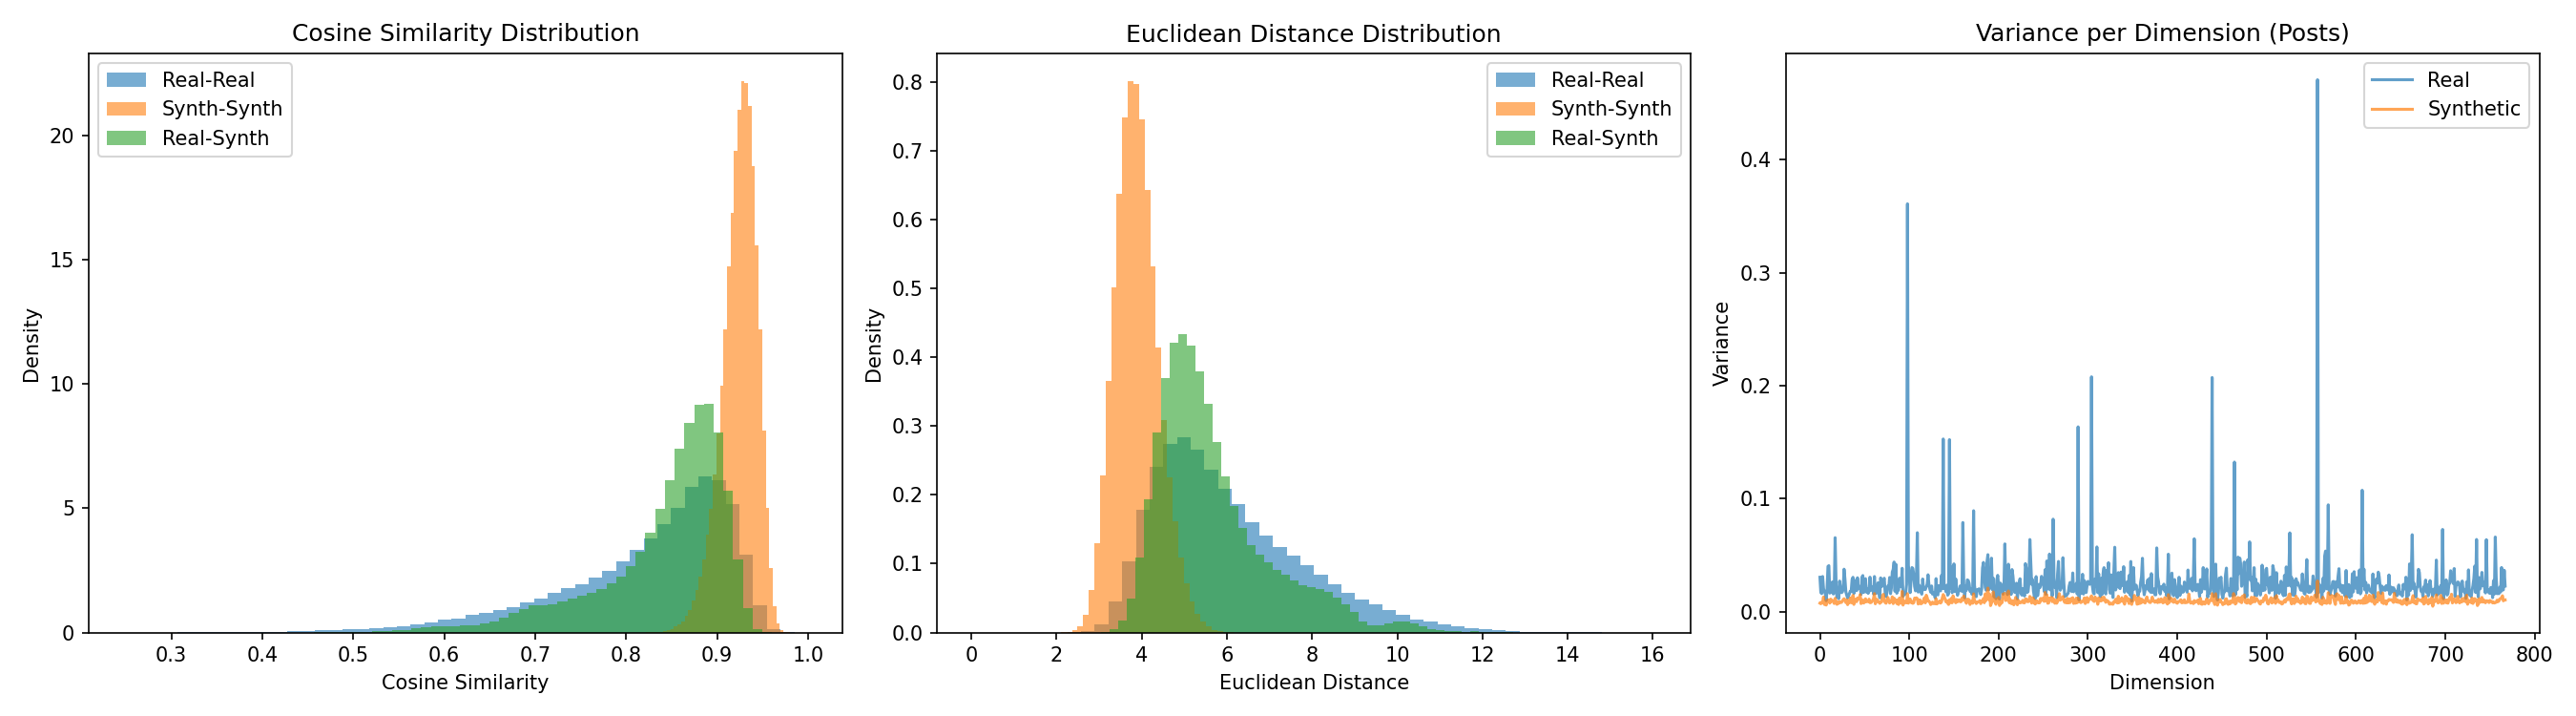
\includegraphics[width=0.9\textwidth]{figures/embedding_comparison.png}
	\caption{Comparison of cosine similarity distributions between real and synthetic embeddings. Synthetic posts cluster tightly with similarities concentrated around 0.90-0.95, while real posts show a broader distribution.}
	\label{fig:embedding_comparison}
\end{figure}

To visualize the embedding space structure, PCA and t-SNE projections were computed for both post and user-level embeddings. Figure~\ref{fig:embedding_visualization_posts} shows the post-level visualization.

\begin{figure}[H]
	\centering
	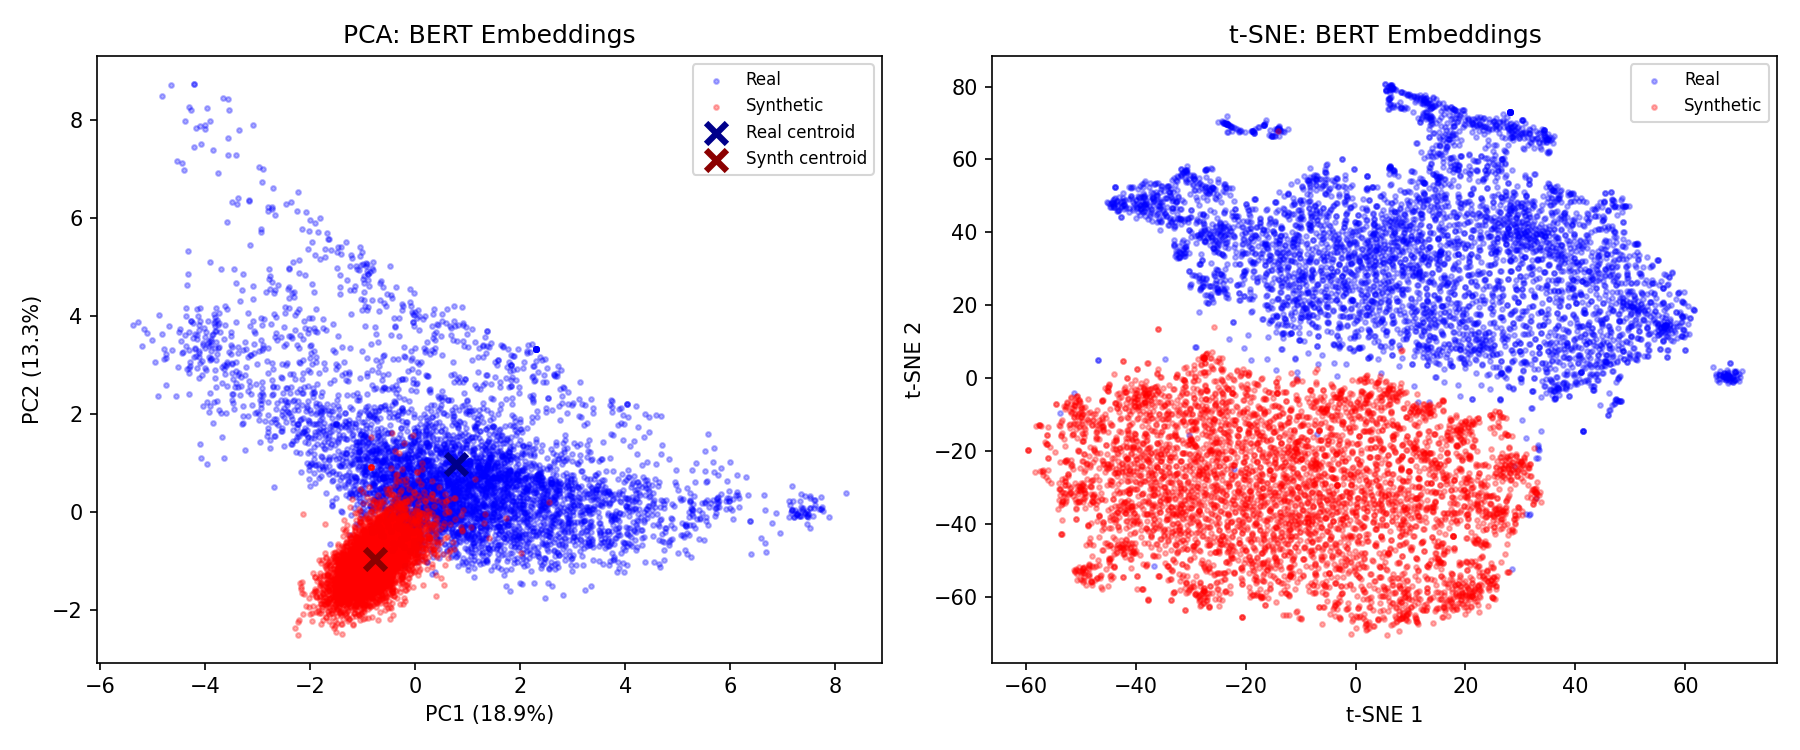
\includegraphics[width=0.95\textwidth]{figures/embeddings_visualization_bert.png}
	\caption{PCA and t-SNE visualization of post embeddings. The synthetic posts (red) form a tight, well-defined cluster, while real posts (blue) spread across a much larger region of the embedding space.}
	\label{fig:embedding_visualization_posts}
\end{figure}

Figure~\ref{fig:embedding_visualization_users} presents the user-level visualization, where the homogeneity of synthetic users becomes even more clear.

\begin{figure}[H]
	\centering
	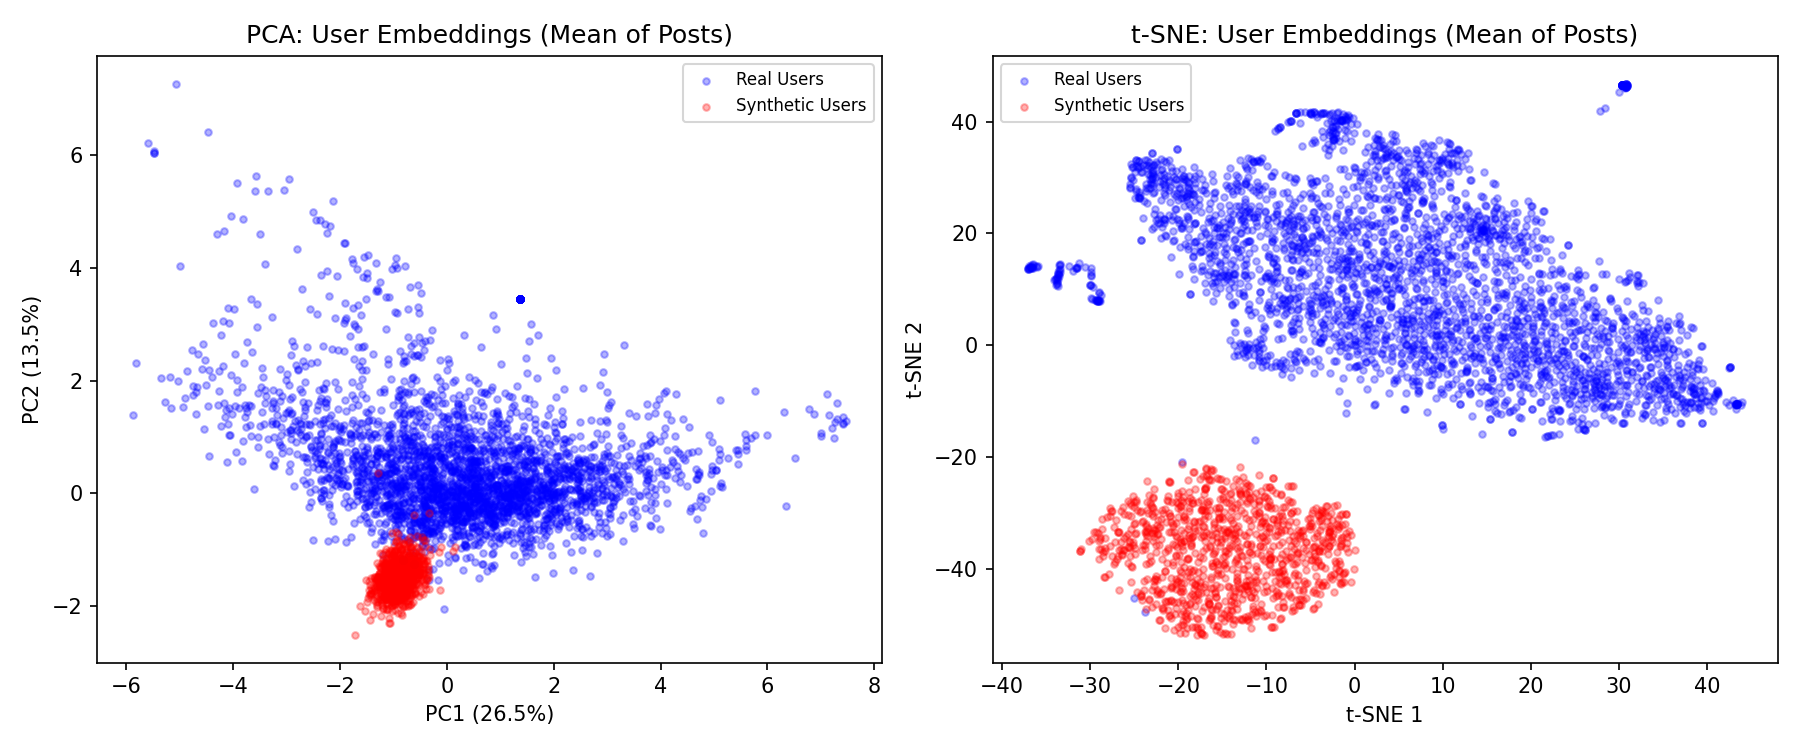
\includegraphics[width=0.95\textwidth]{figures/user_embeddings_visualization.png}
	\caption{PCA and t-SNE visualization of user embeddings (mean of posts per user). Synthetic users (red) cluster in an extremely tight region, while real users (blue) occupy a much broader space.}
	\label{fig:embedding_visualization_users}
\end{figure}

\subsection*{Variance Analysis}

Table \ref{tab:variance_comparison} provides a detailed comparison of variance metrics for both posts and users.

\begin{table}[H]
	\centering
	\caption{Variance comparison: Real vs Synthetic (posts and users)}
	\label{tab:variance_comparison}
	\begin{tabular}{lrrr}
		\toprule
		\textbf{Level}                      & \textbf{Real}            & \textbf{Synthetic} & \textbf{Ratio} \\
		\midrule
		Posts within-group variance         & 0.0264                   & 0.0099             & 2.67x          \\
		Users within-group variance         & 0.0174                   & 0.0015             & 11.23x         \\
		\midrule
		Posts cross-group centroid distance & \multicolumn{3}{c}{2.61}                                       \\
		Users cross-group centroid distance & \multicolumn{3}{c}{2.57}                                       \\
		\bottomrule
	\end{tabular}
\end{table}

The variance per embedding dimension reveals a significant difference in the representational space. For posts, the variance ratio (real/synthetic) is \textbf{2.67x}, with real posts showing a mean variance of \textbf{0.0264} per dimension compared to \textbf{0.0099} for synthetic posts.

At the user level, the disparity is even more pronounced. Table~\ref{tab:variance_comparison} presents the variance comparison for both posts and users.

We distinguish between two types of variance metrics:
\begin{itemize}
	\item \textbf{Within-group variance}: measures how much embeddings vary \textit{within} each group. For example, real user within-group variance (0.0174) indicates how much real users differ from each other. The ratio of 11.23x means synthetic users are much more homogeneous than real users.
	\item \textbf{Cross-group centroid distance}: measures the Euclidean distance between the centroids (mean embeddings) of the two groups. A distance of 2.57 for users indicates that real and synthetic users occupy distinct but not extremely distant regions of the embedding space.
\end{itemize}

% \begin{figure}[H]
% 	\centering
% 	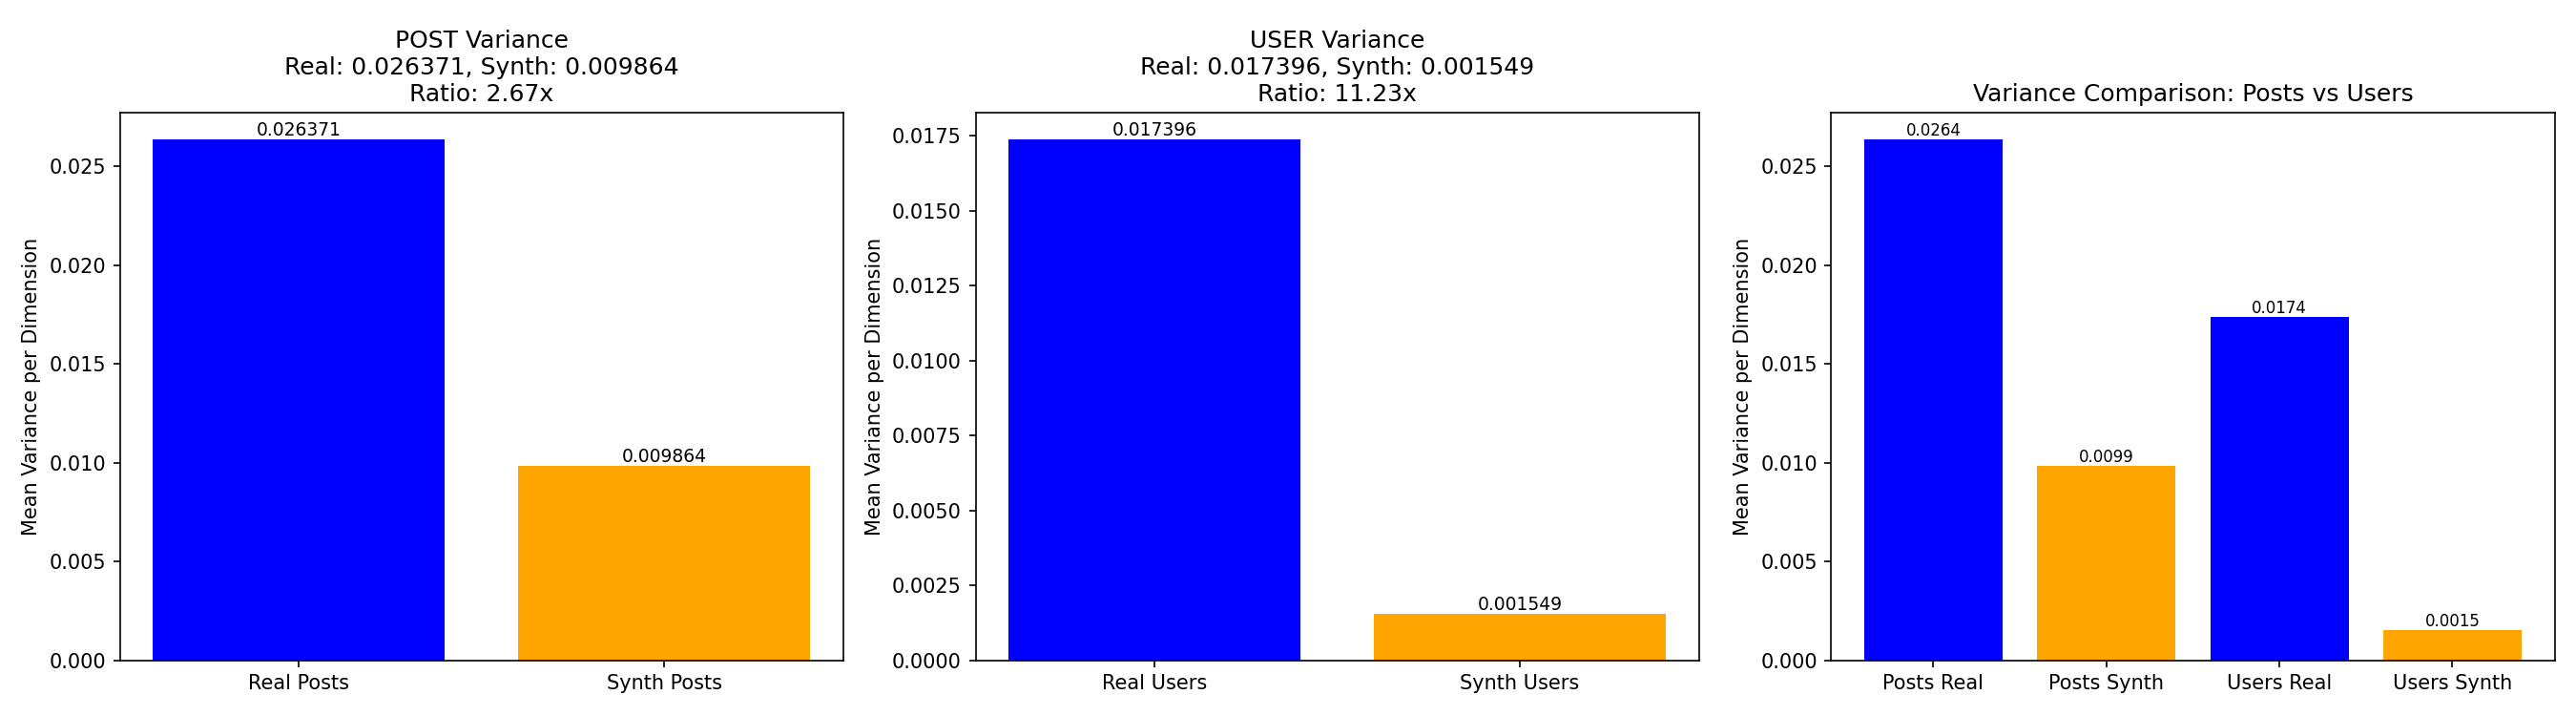
\includegraphics[width=0.95\textwidth]{figures/embedding_variance_summary.png}
% 	\caption{Variance comparison for posts and users. The left panel shows post-level variance, the center shows user-level variance, and the right panel provides a direct comparison. Synthetic data exhibits dramatically lower variance at both levels.}
% 	\label{fig:variance_summary}
% \end{figure}



\subsection*{User-Level Embedding Aggregation}

When aggregating post embeddings by user (computing the mean embedding for each user's posts), the homogeneity becomes even more pronounced. Table~\ref{tab:user_embedding_stats} presents the user-level statistics for both real and synthetic users.

\begin{table}[H]
	\centering
	\caption{User-level embedding statistics: Real vs Synthetic users}
	\label{tab:user_embedding_stats}
	\begin{tabular}{lrr}
		\toprule
		\textbf{Metric}                      & \textbf{Real}             & \textbf{Synthetic} \\
		\midrule
		Total users                          & 25583                    & 1,000              \\
		User-User cosine similarity (mean)   & 0.872                     & 0.988              \\
		User-User cosine similarity (std)    & 0.083                     & 0.004              \\
		Within-group variance (mean per dim) & 0.0174                    & 0.0015             \\
		Cross-group cosine similarity (mean) & \multicolumn{2}{c}{0.893}                      \\
		\bottomrule
	\end{tabular}
\end{table}

The cross-group cosine similarity of \textbf{0.893} indicates moderate semantic similarity between real and synthetic users. However, the within-group metrics reveal stark differences: synthetic users have a within-group cosine similarity of \textbf{0.988} with standard deviation of only 0.004, meaning they are nearly indistinguishable from each other. Real users, in contrast, show a mean similarity of \textbf{0.872} with much higher variance (std=\textbf{0.083}), reflecting natural diversity in content and interests, even though they are still relatively similar on average.

% \begin{figure}[H]
% 	\centering
% 	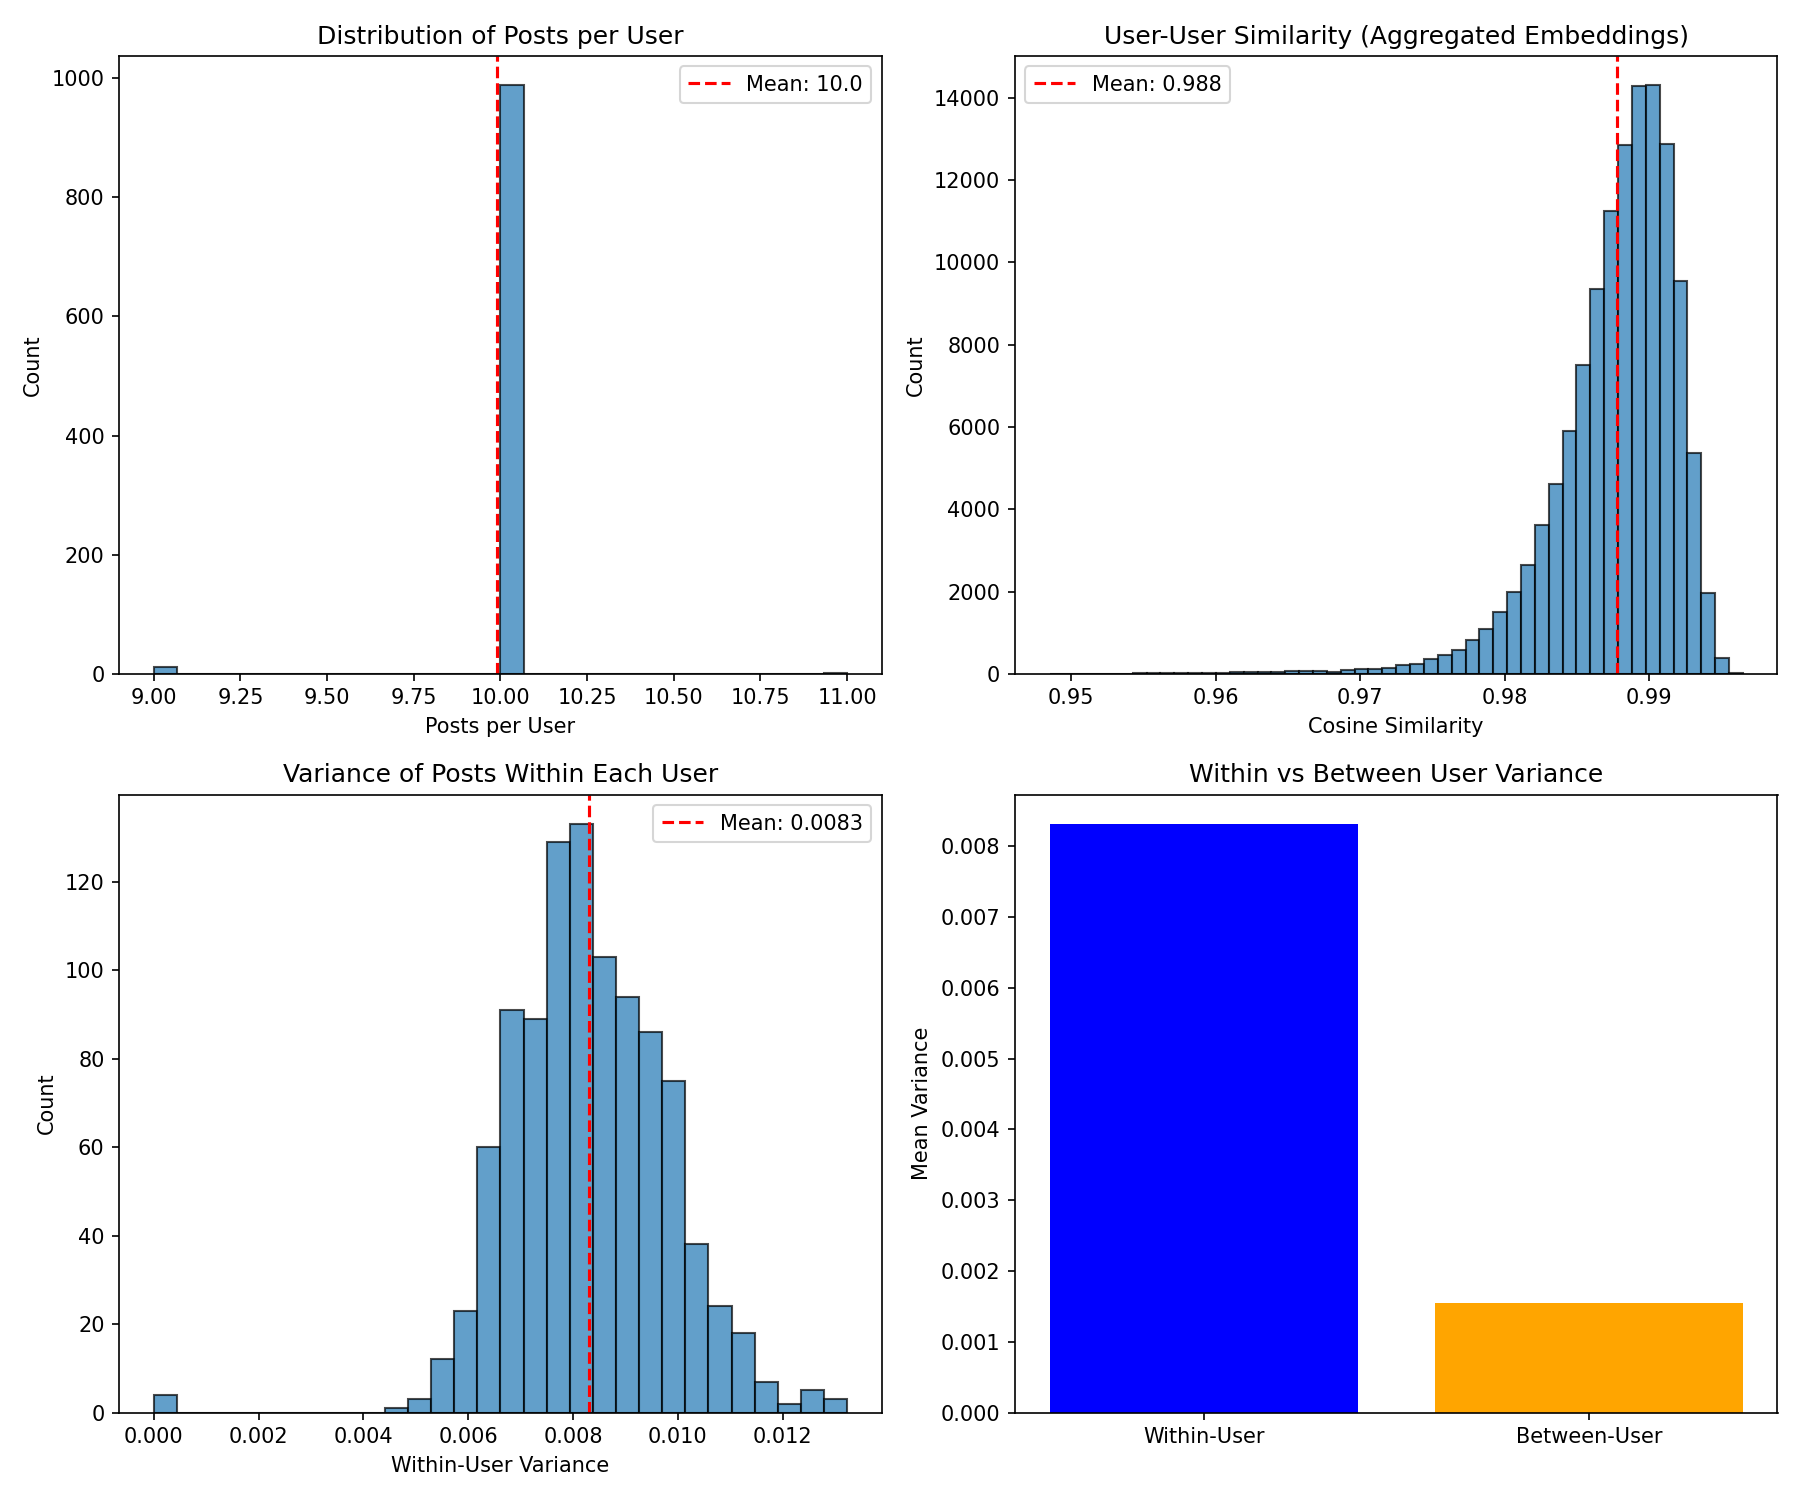
\includegraphics[width=0.9\textwidth]{figures/user_embedding_analysis.png}
% 	\caption{User embedding analysis showing the distribution of posts per user, cosine similarity between users, and variance decomposition. The extremely high user similarity (0.988) indicates synthetic users lack diversity.}
% 	\label{fig:user_embedding}
% \end{figure}

% \subsection*{Nearest Neighbors Analysis}

% To further investigate the embedding space structure, a nearest neighbors analysis was performed. Figure~\ref{fig:nearest_neighbors} shows the composition of nearest neighbors for both real and synthetic posts.

% \begin{figure}[H]
% 	\centering
% 	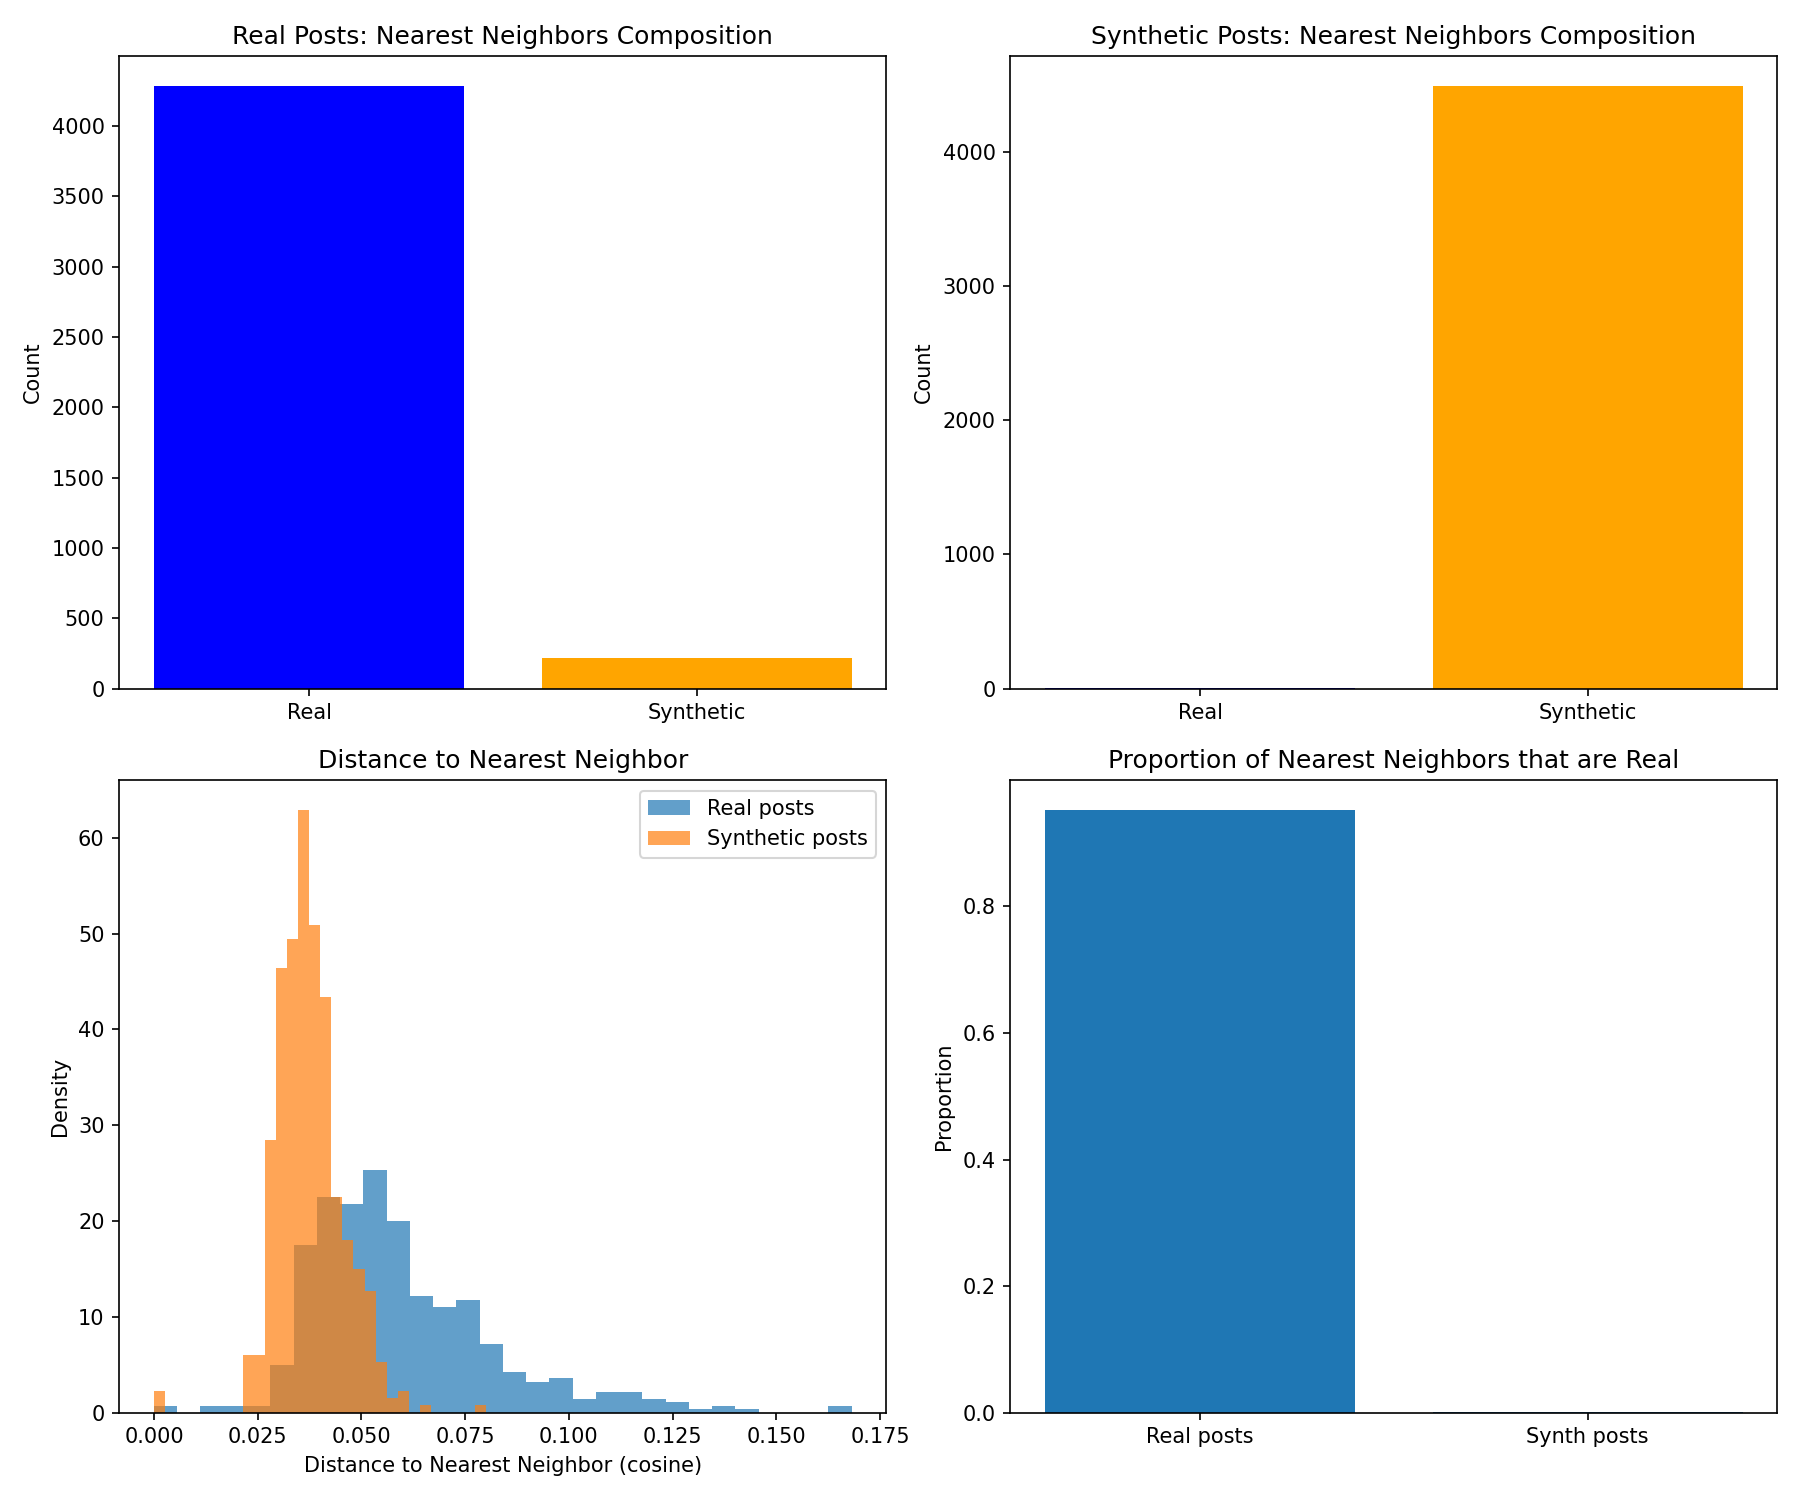
\includegraphics[width=0.9\textwidth]{figures/nearest_neighbors_analysis.png}
% 	\caption{Nearest neighbors composition: Real posts find 95\% of their neighbors among other real posts, while synthetic posts find 99.9\% of their neighbors among other synthetic posts, forming an isolated cluster.}
% 	\label{fig:nearest_neighbors}
% \end{figure}

% The analysis reveals a stark separation:
% \begin{itemize}
% 	\item \textbf{Real posts}: 95.2\% of nearest neighbors are other real posts
% 	\item \textbf{Synthetic posts}: 99.9\% of nearest neighbors are other synthetic posts
% \end{itemize}

% This confirms that synthetic posts form an isolated cluster in the embedding space, disconnected from the real data distribution. This isolation may cause issues during inference, as the model encounters out-of-distribution embeddings.

% \subsection*{Implications for Link Prediction}

% The embedding analysis reveals several challenges for the link prediction task:

% \begin{enumerate}
% 	\item \textbf{Homogeneity}: Synthetic nodes are too similar to each other, making it difficult for the model to learn meaningful distinctions
% 	\item \textbf{Isolation}: Synthetic embeddings form a separate cluster, disconnected from real embeddings
% 	\item \textbf{OOD Risk}: When predicting links involving synthetic nodes, the model operates on out-of-distribution data
% \end{enumerate}

% Potential mitigation strategies include:
% \begin{itemize}
% 	\item Regenerating synthetic posts with more diverse prompts
% 	\item Adding noise to synthetic embeddings to increase variance
% 	\item Connecting synthetic nodes to real nodes in the graph structure
% 	\item Using higher probability thresholds (0.7-0.8) for filtering predictions
% \end{itemize}


% \section{Summary}

% The data understanding phase revealed a rich dataset of 182,545 posts from the Gab social network, spanning nearly a decade (2016-2025). Key findings include:

% \begin{itemize}
% 	\item \textbf{Growth pattern}: The platform shows exponential growth, with 2025 data alone representing 68\% of all posts
% 	\item \textbf{Language homogeneity}: 97\% English content, making it suitable for single-language NLP tasks
% 	\item \textbf{Content characteristics}: Short-form content dominates (median 89 characters, 13 words) with heavy-tailed distributions
% 	\item \textbf{Engagement patterns}: Highly skewed distributions with 28\% zero-engagement posts and viral outliers reaching 20,000+ interactions
% 	\item \textbf{User dynamics}: Power-law distribution with 0.43\% of users (116 power users) driving significant content volume
% 	\item \textbf{Data quality}: High completeness (99.52\%) with only the \texttt{language} field showing missing values; perfect snapshot-incremental consistency
% 	\item \textbf{Duplicate trend}: Increasing content duplication over time (from 1.79\% to 10.04\%), suggesting potential bot activity or viral content resharing
% 	\item \textbf{Embedding quality}: Synthetic embeddings show extreme homogeneity (cosine sim 0.925 vs 0.821 for real) and form an isolated cluster, posing challenges for link prediction
% \end{itemize}

% The dataset is well-suited for link prediction and social network analysis tasks, with the temporal snapshots enabling longitudinal studies of network evolution. The preprocessing pipeline should address the minor missing values, consider strategies for handling the heavy-tailed engagement distributions, and account for the embedding homogeneity in synthetic data.
